%----------------------------------------------------------------------------
%----------------------------------------------------------------------------
%				    	SETUP
%----------------------------------------------------------------------------
%----------------------------------------------------------------------------

\documentclass[11pt]{article}

%----------------------------------------------------------------------------
%			  	   PACKAGES
%----------------------------------------------------------------------------

%%%%%%%%%%%%%%%%%%%%%%%
% 	  Packages
%%%%%%%%%%%%%%%%%%%%%%%

%% Fonts and Symbols
%% --------------------------
\usepackage{
	amsmath,			% math operators
	amssymb,			% math symbols
	%			amsthm,				% theorem environment
	soul,				% strike through with \st{}
	xcolor,				% color!
	%			xfrac,				% fancy fractions
}	

\definecolor{mygreen}{rgb}{0,0.6,0}
\definecolor{mygray}{rgb}{0.5,0.5,0.5}
\definecolor{mymauve}{rgb}{0.58,0,0.82}
\definecolor{darkblue}{rgb}{0,0,0.4}	

%% Graphics
%% --------------------
\usepackage{
			graphicx,			% allows insertion of images
			subfigure,			% allows subfigures (a), (b), etc.
}				
\graphicspath{ {graphics/} }	% (graphicx) relative path to graphics folder				

%% Tables
%% --------------------------
\usepackage{
			booktabs,			% better tables, discourages vertical rulings
			multicol,			% allow multi columns
%			tocloft,			% finer control over TOC; enabled below due to subfigure conflict
}
%\usepackage[subfigure]{tocloft}
%\addtocontents{toc}{\cftpagenumbersoff{subsubsection}} % turn off subsubsection page numbers in ToC

%% Layout Alteration
%% --------------------------
\usepackage{			
%			caption,			% line breaks in captions with \\
%			changepage,			% change margins for PARTS of pages with (adjustwidth)
			fancyhdr,			% see config in LAYOUT AND STYLING
			framed,				% nice boxes; used in Supervisor's Approval
%			fullpage,			% set full page margins
			geometry,			% change the margins for specific PAGES
%			lastpage,			% used with (fancyhdr)
			parskip,			% disable indents
			pdflscape,			% ???
			rotating,			% sideways figures
}
\geometry{						% specify page size options for (geometry)
	a4paper, 			% paper size
	hmargin=1in,		% horizontal margins
	vmargin=1in,		% vertical margins
}	


%% Units
%% --------------------------
\usepackage{
	siunitx,			% has S (decimal align) column type
}
\sisetup{input-symbols = {()},  % do not treat "(" and ")" in any special way
		group-digits  = false, 	% no grouping of digits
%		load-configurations = abbreviations,
%		per-mode = symbol,
}

%% Misc
%% --------------------------
\usepackage{
	enumitem,			% better control of enumerations, descriptions, etc
	listings,			% source code import and display
}

\lstset{ %
	language=verilog,				% the language of the code
	basicstyle=\footnotesize,       % the size of the fonts that are used for the code
	numbers=none,                   % where to put the line-numbers
	numberstyle=\tiny\color{mygray},% the style that is used for the line-numbers
	stepnumber=1,                   % the step between two line-numbers. If it's 1, each line
	% 	will be numbered
	numbersep=5pt,                  % how far the line-numbers are from the code
	backgroundcolor=\color{white},  % choose the background color. You must add \usepackage{color}
	showspaces=false,               % show spaces adding particular underscores
	showstringspaces=false,         % underline spaces within strings
	showtabs=false,                 % show tabs within strings adding particular underscores
	frame=single,	                % box the code [single, none]
	rulecolor=\color{black},        % if not set, the frame-color may be changed on line-breaks
	% 	within not-black text (e.g. commens (green here))
	tabsize=2,                      % sets default tabsize to 2 spaces
	captionpos=b,                   % sets the caption-position to bottom
	breaklines=true,                % sets automatic line breaking
	breakatwhitespace=false,        % sets if automatic breaks should only happen at whitespace
	title=\lstname,                 % show the filename of files included with \lstinputlisting;
	% 	also try caption instead of title
	keywordstyle=[1]\bfseries\color{darkblue},    % keyword style for mnemonics
	keywordstyle=[2]\bfseries\color{violet},	% keyword style for . mnemonics
	commentstyle=\color{mygreen},   % comment style
	stringstyle=\color{mymauve},    % string literal style
	escapeinside={\%*}{*)},         % if you want to add a comment within your code
	morekeywords={*,...}           	% if you want to add more keywords to the set
}

%----------------------------------------------------------------------------
%		     MACROS AND COMMANDS
%----------------------------------------------------------------------------

% Defines a new command for the horizontal lines, change thickness here
\newcommand{\HRule}{\rule{\linewidth}{0.5mm}} 

% override S column type with centered text column
\newcommand{\textcol}[1]{\multicolumn{1}{c}{#1}}


%----------------------------------------------------------------------------
%----------------------------------------------------------------------------
%				   DOCUMENT
%----------------------------------------------------------------------------
%----------------------------------------------------------------------------

\begin{document}

%----------------------------------------------------------------------------
%				    TITLE PAGE
%----------------------------------------------------------------------------

\begin{titlepage}

\center
 
% Header
\textsc{\LARGE University of Victoria}\\[1cm] 	% Name of your university/college
\textsc{\Large CENG 241}\\[0.5cm] 			% Major heading such as course name
\textsc{\large Digital Design I}\\[0.5cm] 		% Minor heading such as course title


% Lab Title
\HRule \\[0.4cm]
{\huge \bfseries Lab 5 - Sequential Circuits: \\Flip-Flops and Counters}\\[0.2cm] % Title of your document
\HRule \\[1.5cm]
 
 
%Lab Instructor Details
\begin{minipage}{0.7\textwidth}
\begin{flushleft} 

\large\emph{Instructor:} \\
Dr. Amirali \textsc{Baniasadi} \\
\vspace{12 pt}
\emph{Teaching Assistant:} \\
Grace \textsc{Hui}

\end{flushleft}
\end{minipage}
~
%% No content here, but it keeps the alignment of the instructor/TA
%% box correct.
%% Consider revising.
\begin{minipage}{0.1\textwidth}
\begin{flushright} \large
%Dr. Barbara \textsc{Sawicka} \\
\vspace{12 pt}
%\emph{Teaching Assistant:} \\
%Vahid \textsc{Moradi}
\end{flushright}
\end{minipage}\\[2cm]


% Lab members
\Large Yves \textsc{S\'en\'echal}
\large V00213837	\\
\Large Tyler \textsc{Stephen}
\large V00812021	\\
A01 - B03\\[1.5cm] 


% Date
{\large \today}\\ % Date, change the \today to a set date if you want to be precise

% Logo
\begin{figure}[b]	 % put logo at bottom of the page
	\centering
	\includegraphics[scale=0.3]{UVic_logo}
\end{figure}

\end{titlepage}

%----------------------------------------------------------------------------
%				    BODY
%----------------------------------------------------------------------------

\section{Introduction}

Sequential logic depends on present and past signals to determine the system's next state, hence sequential circuits have memory. The SR latches, D flip flops, T flip flops, and counters are examples of sequential circuits; they will be explored in this lab.

\section{555 Timer}

The required duty cycle of 50\% and frequency of a few hertz were obtained from using resistors $R_a = 330\Omega$, $R_b = 1M\Omega$  and a capacitor $C = 0.1\mu\Omega$. From the following formulas,
\[
       Clock\\\ frequency=\frac { 1.44 }{ ({ R }_{ a }+2{ R }_{ b })C } 
\]
\[
       Duty\\\ cycle=\frac { { R }_{ a }+{ R }_{ b } }{ { R }_{ a }+2{ R }_{ b } } 
\]
the expected clock frequency and duty cycle was calculated to be 7.2Hz and 50\% respectfully. Figure \ref{fig:timer} shows the experimental frequency of 8.2Hz with a duty cycle of 54.08\%. Resistance and capacitance in the leads may account for these discrepancies. 


\begin{figure}[htpb]
	\centering
	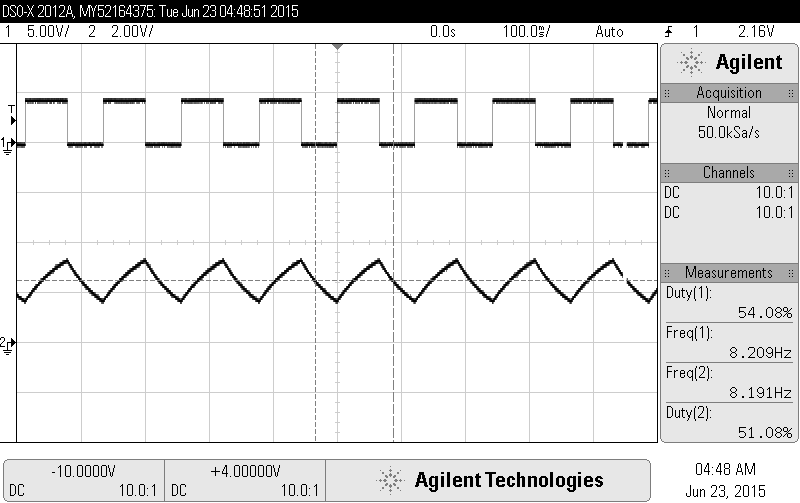
\includegraphics[width=0.95\textwidth]{timer}
	\caption{Output of the timer pin (top) and capacitor pin (bottom) for a 555 timer}
	\label{fig:timer}
\end{figure}

\section{RS Latch}
\begin{itemize}
	\item schematic of latch with two inverters on output
	\item screenshot of oscillations at 00/11
	\item how does frequency of oscilations relate to delay in circuit?
\end{itemize}

\begin{figure}[htpb]
	\centering
	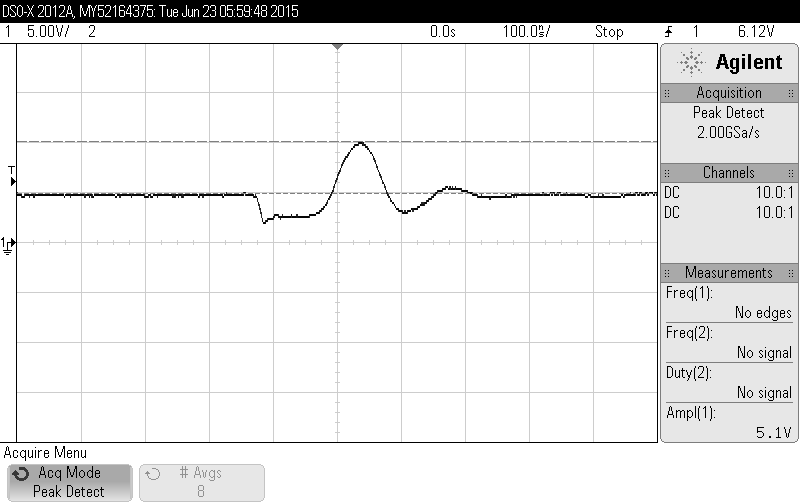
\includegraphics[width=0.95\textwidth]{rs_latch}
	\caption{Oscillatory output of an RS latch in the indeterminate state}
	\label{fig:rs_latch}
\end{figure}

\section{D Flip-Flop}
\begin{itemize}
	\item screenshot of D-FF changing on negative edge
	\item description of how D-FF works
\end{itemize}

\begin{figure}[htpb]
	\centering
	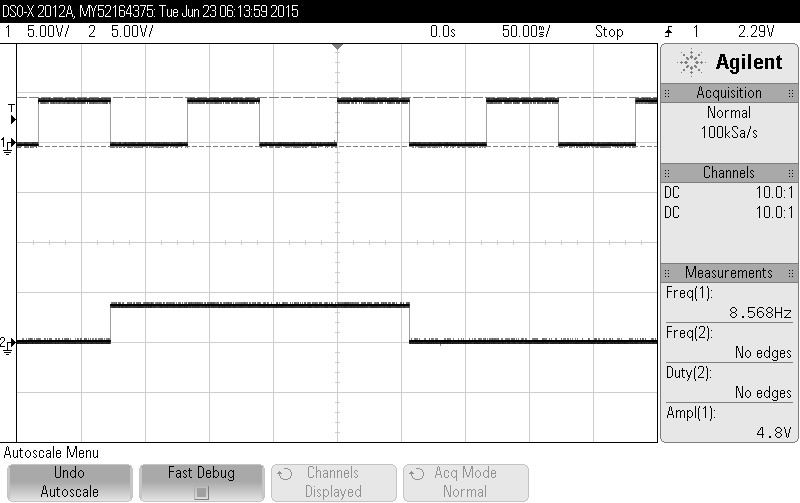
\includegraphics[width=0.95\textwidth]{d-ff}
	\caption{The D flip-flop only updates its value on the falling edge}
	\label{fig:d-ff}
\end{figure}

\section{T Flip-Flop}
\begin{itemize}
	\item screenshot for T=1
\end{itemize}

\begin{figure}[htpb]
	\centering
	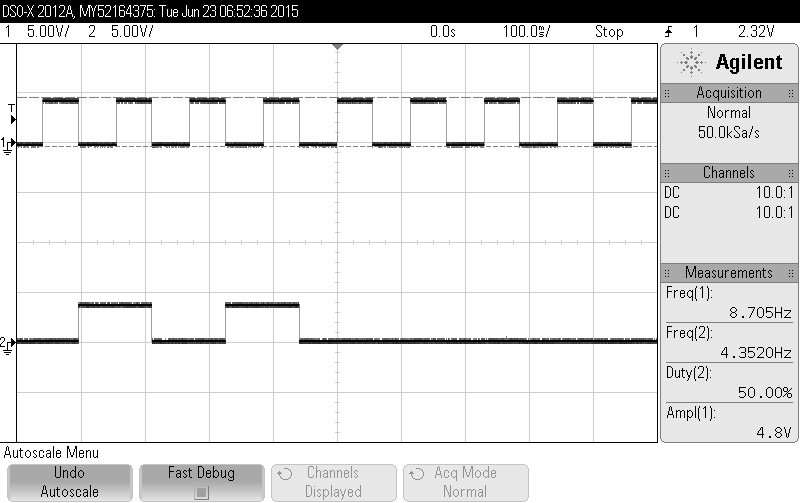
\includegraphics[width=0.95\textwidth]{t-ff}
	\caption{Output of a T flip-flop for $T=1$}
	\label{fig:t-ff}
\end{figure}

\section{Counter}
\begin{itemize}
	\item schematic of circuit as built in lab
	\item Explain why the output of the circuit is not in the range of 3 to 12 in the first few clock cycles.
\end{itemize}

\begin{figure}[htpb]
	\centering
	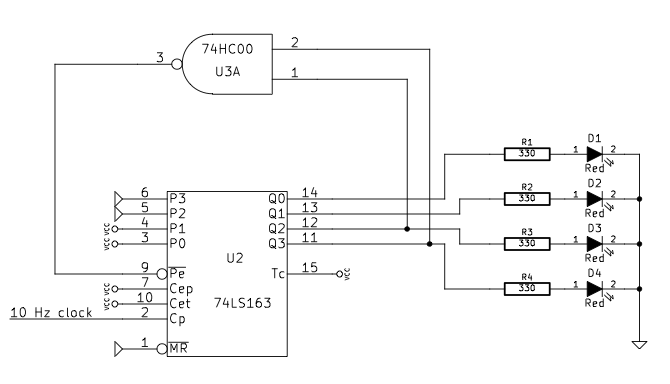
\includegraphics[width=0.95\textwidth]{schematic_counter}
	\caption{74LS163 used to count 3 to 12 before resetting}
	\label{fig:counter}
\end{figure}

\section{Conclusion}

\end{document}